\chapter{Diseño del Proyecto}

\section{Stack Tecnológico}

\begin{longtable}{>{\bfseries}p{3cm} p{4cm} p{5.5cm}}
  \toprule
  \textbf{Capa} & \textbf{Tecnología} & \textbf{Justificación} \\
  \midrule
  \endhead
  Mobile         & React Native + Expo SDK 52+   & Android, OTA updates vía EAS \\[3pt]
  Web            & Expo Router (web) & Misma codebase, rutas públicas en browser \\[3pt]
  Lenguaje       & TypeScript                    & Tipado estático, seguridad en desarrollo \\[3pt]
  BaaS           & Supabase (free tier)          & PostgreSQL + Auth + Storage + Realtime sin servidor \\[3pt]
  Cliente BaaS   & supabase-js v2                & SDK oficial, soporte completo \\[3pt]
  Base Datos  & PostgreSQL (vía Supabase)     & Modelo relacional, consistencia transaccional, RLS \\[3pt]
  Auth           & Supabase Auth                 & JWT, roles vía \texttt{user\_metadata}, sesiones anónimas \\[3pt]
  Storage        & Supabase Storage              & Bucket \texttt{menu-imgs} (CDN público) \\[3pt]
  Tiempo real    & Supabase Realtime             & Canal \texttt{orders} y \texttt{table\_calls} \\[3pt]
  Reportes       & PostgreSQL functions + RPC    & Agregaciones server-side \\[3pt]
  Pagos QR       & QR estático banco/billetera   & Sin pasarela; verificación manual por admin \\[3pt]
  Deploy         & Expo EAS Build + EAS Update   & Build nativo y OTA sin pasar por stores \\[3pt]
  Versiones      & Git + GitHub                  & Branching por feature, PRs obligatorios \\
  \bottomrule
  \caption{Stack tecnológico del sistema}
\end{longtable}

\clearpage

\section{Modelo de Datos}

\subsection{Entidades y Relaciones}

El sistema define las siguientes entidades principales y sus relaciones:

\begin{figure}[H]
    \centering
    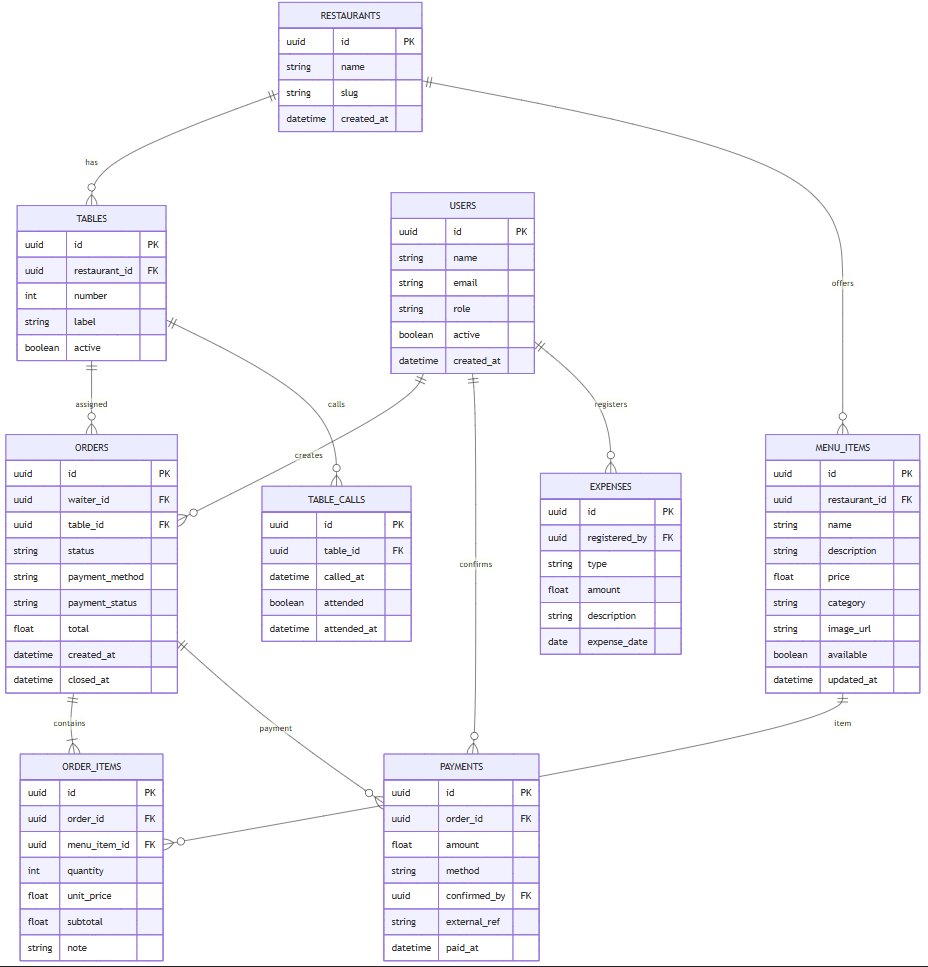
\includegraphics[width=0.95\textwidth]{img/erd_database.png}
    \caption{Modelo entidad–relación de la base de Datos}
    \label{fig:erd_database}
\end{figure}

\clearpage

\subsection{Esquema de Tablas}

A continuación se describe cada tabla del modelo de datos:

\vspace{6pt}
\noindent\textbf{\texttt{restaurants}}

\begin{tabular}{lll}
  \toprule
  \textbf{Campo} & \textbf{Tipo} & \textbf{Descripción} \\
  \midrule
  \texttt{id}         & uuid        & PK \\
  \texttt{name}       & text        & Nombre del restaurante \\
  \texttt{slug}       & text UNIQUE & Identificador en URLs públicas \\
  \texttt{created\_at} & timestamptz & Fecha de creación \\
  \bottomrule
\end{tabular}

\vspace{6pt}
\noindent\textbf{\texttt{tables}}

\begin{tabular}{lll}
  \toprule
  \textbf{Campo} & \textbf{Tipo} & \textbf{Descripción} \\
  \midrule
  \texttt{id}            & uuid    & PK \\
  \texttt{restaurant\_id} & uuid FK & Referencia a \texttt{restaurants} \\
  \texttt{number}        & integer & Número de mesa \\
  \texttt{label}         & text    & Nombre descriptivo (ej: ``Terraza 3'') \\
  \texttt{active}        & boolean & Estado activo/inactivo \\
  \bottomrule
\end{tabular}

\vspace{6pt}
\noindent\textbf{\texttt{users}}

\begin{tabular}{lll}
  \toprule
  \textbf{Campo} & \textbf{Tipo} & \textbf{Descripción} \\
  \midrule
  \texttt{id}         & uuid            & PK (sincronizado con \texttt{auth.users}) \\
  \texttt{name}       & text            & Nombre del usuario \\
  \texttt{email}      & text UNIQUE     & Correo electrónico \\
  \texttt{role}       & enum            & \texttt{waiter} | \texttt{admin} \\
  \texttt{active}     & boolean         & Estado de la cuenta \\
  \texttt{created\_at} & timestamptz    & Fecha de registro \\
  \bottomrule
\end{tabular}

\begin{notabox}
\texttt{password\_hash} se omite: Supabase Auth gestiona credenciales internamente.
El campo \texttt{role} se sincroniza hacia \texttt{auth.users.raw\_user\_meta\_data}
mediante un trigger \texttt{AFTER UPDATE}.
\end{notabox}

\vspace{6pt}
\noindent\textbf{\texttt{menu\_items}}

\begin{tabular}{lll}
  \toprule
  \textbf{Campo} & \textbf{Tipo} & \textbf{Descripción} \\
  \midrule
  \texttt{id}            & uuid          & PK \\
  \texttt{restaurant\_id} & uuid FK      & Referencia a \texttt{restaurants} \\
  \texttt{name}          & text          & Nombre del platillo \\
  \texttt{description}   & text          & Descripción \\
  \texttt{price}         & decimal(10,2) & Precio \\
  \texttt{category}      & text          & Categoría \\
  \texttt{image\_url}    & text          & URL del CDN de Storage \\
  \texttt{available}     & boolean       & Disponibilidad en tiempo real \\
  \texttt{updated\_at}   & timestamptz   & Última actualización \\
  \bottomrule
\end{tabular}

\vspace{6pt}
\noindent\textbf{\texttt{orders}}

\begin{tabular}{lll}
  \toprule
  \textbf{Campo} & \textbf{Tipo} & \textbf{Descripción} \\
  \midrule
  \texttt{id}             & uuid          & PK \\
  \texttt{waiter\_id}     & uuid FK       & Referencia a \texttt{users} \\
  \texttt{table\_id}      & uuid FK       & Referencia a \texttt{tables} \\
  \texttt{status}         & enum          & \texttt{pending | ready | delivered | cancelled} \\
  \texttt{payment\_method} & enum         & \texttt{cash | qr} \\
  \texttt{payment\_status} & enum         & \texttt{pending | confirmed} \\
  \texttt{total}          & decimal(10,2) & Total de la orden \\
  \texttt{created\_at}    & timestamptz   & Fecha de apertura \\
  \texttt{closed\_at}     & timestamptz   & Asignado automáticamente al entregar \\
  \bottomrule
\end{tabular}

\vspace{6pt}
\noindent\textbf{\texttt{order\_items}}

\begin{tabular}{lll}
  \toprule
  \textbf{Campo} & \textbf{Tipo} & \textbf{Descripción} \\
  \midrule
  \texttt{id}           & uuid          & PK \\
  \texttt{order\_id}    & uuid FK       & Referencia a \texttt{orders} \\
  \texttt{menu\_item\_id} & uuid FK     & Referencia a \texttt{menu\_items} \\
  \texttt{quantity}     & integer       & Cantidad \\
  \texttt{unit\_price}  & decimal(10,2) & Snapshot del precio al momento del pedido \\
  \texttt{subtotal}     & decimal(10,2) & Subtotal \\
  \texttt{note}         & text          & Indicación especial del cliente \\
  \bottomrule
\end{tabular}   

\vspace{6pt}
\noindent\textbf{\texttt{payments}}

\begin{tabular}{lll}
  \toprule
  \textbf{Campo} & \textbf{Tipo} & \textbf{Descripción} \\
  \midrule
  \texttt{id}           & uuid          & PK \\
  \texttt{order\_id}    & uuid FK       & Referencia a \texttt{orders} \\
  \texttt{amount}       & decimal(10,2) & Monto pagado \\
  \texttt{method}       & enum          & \texttt{cash | qr} \\
  \texttt{confirmed\_by} & uuid FK      & Admin que confirmó el pago \\
  \texttt{external\_ref} & text         & Reservado para pasarela futura \\
  \texttt{paid\_at}     & timestamptz   & Fecha/hora del pago \\
  \bottomrule
\end{tabular}

\vspace{6pt}
\noindent\textbf{\texttt{expenses}}

\begin{tabular}{lll}
  \toprule
  \textbf{Campo} & \textbf{Tipo} & \textbf{Descripción} \\
  \midrule
  \texttt{id}             & uuid          & PK \\
  \texttt{registered\_by} & uuid FK       & Usuario que registró el gasto \\
  \texttt{type}           & text          & Tipo de gasto \\
  \texttt{amount}         & decimal(10,2) & Monto \\
  \texttt{description}    & text          & Descripción \\
  \texttt{expense\_date}  & date          & Fecha del gasto \\
  \bottomrule
\end{tabular}

\clearpage
\noindent\textbf{\texttt{table\_calls}}

\begin{tabular}{lll}
  \toprule
  \textbf{Campo} & \textbf{Tipo} & \textbf{Descripción} \\
  \midrule
  \texttt{id}          & uuid        & PK \\
  \texttt{table\_id}   & uuid FK     & Referencia a \texttt{tables} \\
  \texttt{called\_at}  & timestamptz & Momento de la llamada \\
  \texttt{attended}    & boolean     & Si fue atendida \\
  \texttt{attended\_at} & timestamptz & Momento de atención \\
  \bottomrule
\end{tabular}

\section{Estructura del Proyecto}

La estructura de directorios del repositorio sigue las convenciones de Expo Router:

\begin{Verbatim}[fontsize=\small, frame=single, framesep=3mm]
gestion-comandas/
|-- app/
|   |-- (auth)/          login.tsx, _layout.tsx
|   |-- (waiter)/        tables/, orders/, _layout.tsx
|   |-- (admin)/         menu/, expenses/, reports/, _layout.tsx
|   |-- menu/[slug].tsx
|   |-- table/[slug]/[tableId].tsx
|   \-- _layout.tsx
|-- components/
|   |-- tables/TableCard.tsx
|   |-- orders/
|   |-- menu/
|   |-- customer/CallWaiterButton.tsx
|   \-- ui/
|-- lib/
|   |-- supabase.ts
|   |-- supabase-public.ts
|   |-- hooks/
|   |   |-- useOrders.ts
|   |   |-- useTables.ts
|   |   |-- useTableCalls.ts
|   |   |-- useMenu.ts
|   |   \-- useReports.ts
|   \-- types/database.types.ts
|-- supabase/
|   |-- migrations/
|   |   |-- 001_schema.sql
|   |   |-- 002_rls.sql
|   |   |-- 003_functions.sql
|   |   \-- 004_triggers.sql
|   \-- config.toml
|-- app.json
|-- eas.json
\-- tsconfig.json
\end{Verbatim}

\section{Roles y Accesos}

\begin{longtable}{p{6cm} ccc}
  \toprule
  \textbf{Funcionalidad} & \textbf{Waiter} & \textbf{Admin} & \textbf{Customer} \\
  \midrule
  \endhead
  Ver menú (solo disponibles)         & \checkmark & \checkmark & carta pública \\
  Ver menú completo (con no disp.)    & \checkmark & \checkmark & \checkmark (anónimo) \\
  Crear pedido                        & \checkmark & \checkmark & --- \\
  Actualizar estado de pedido         & \checkmark & \checkmark & --- \\
  Confirmar pago QR                   & ---        & \checkmark & --- \\
  Vista de estado de mesas            & \checkmark & --- & --- \\
  Recibir notificación de llamada     & \checkmark & --- & --- \\
  Llamar al mesero                    & ---        & --- & \checkmark \\
  Gestionar menú (CRUD + imágenes)    & ---        & \checkmark & --- \\
  Registrar gastos                    & ---        & \checkmark & --- \\
  Ver reportes financieros            & ---        & \checkmark & --- \\
  Ver ranking de platos más vendidos  & ---        & \checkmark & --- \\
  Gestionar usuarios                  & ---        & \checkmark & --- \\
  Carta digital (pública, sin auth)   & ---        & --- & --- \\
  \bottomrule
  \caption{Matriz de roles y accesos del sistema}
\end{longtable}